\section{Auswertung}
\label{sec:Auswertung}

\raggedright

Im Folgenden wird die Auswertung der verschiedenen Messungen präsentiert. Die Fehlerrechnungen und Ausgleichsrechnungen werden mittels \textit{Python} durchgeführt.
Für die verwendeten physikalischen Konstanten wurde die \textit{Python}-Bibliothek \textit{SciPy} \cite{scipy} verwendet.

\subsection{Magnetfeldmessung}

Als erstes wird die Messung des Magnetfeldes betrachtet. In Tabelle \ref{tab:magnetfeld} sind die Magnetfeldstärken $B$ in Abhängigkeit von der Position $z$ der Hall-Sonde aufgeführt.
Der höchste Wert des Magnetfeldes entspricht $B_{\mathrm{max}}=\SI{419}{\milli\tesla}$, welcher als Wert innerhalb der Probe angenommen wird und in der nachfolgenden Auswertung verwendet wird.

\begin{table}
  \centering
  \begin{tabular}{c c c c}
    \toprule
    $z$ / mm & $B$ / mT & $z$ / mm & $B$ / mT\\
    \midrule
        70  &  3   &  96   & 413  \\
        75  &  16  &  97   & 408  \\
        80  &  76  &  98   & 401  \\
        81  &  107 &  99   & 392  \\
        82  &  149 &  100  & 380  \\
        83  &  197 &  101  & 362  \\
        84  &  255 &  102  & 337  \\
        85  &  320 &  103  & 307  \\
        86  &  357 &  104  & 262  \\
        87  &  378 &  105  & 201  \\
        88  &  392 &  106  & 155  \\
        89  &  401 &  107  & 113  \\
        90  &  407 &  108  & 80   \\
        91  &  410 &  109  & 56   \\
        92  &  413 &  110  & 39   \\
        93  &  414 &  115  & 8    \\
        94  &  419 &  120  & 2    \\
        95  &  416 &       &      \\
    \bottomrule
  \end{tabular}
  \caption{Gemessene Magnetfeldstärke $B$ in Abhängigkeit der Position $z$ der Hall-Sonde.}
  \label{tab:magnetfeld}
\end{table}

\subsection{Messung der dotierten GaAs-Proben}

Die Dicke $L$ der Proben und ihre Dotierung $N$ sind in Tabelle \ref{tab:ln} aufgelistet.
Zunächst werden die gemessenen Winkel in Radialmaß umgerechnet und mittels
\begin{align}
  \theta = \frac{1}{2}(\theta_1 - \theta_2)
\end{align}
die Faradayrotation bestimmt.
Dabei entspricht $\theta_1$ und $\theta_2$ den gemessenen Winkeln in Abhängikeit von den Wellenlängen der Filter und der Polung des Magnetfeldes.
Die Faradayrotation wird anschließend über die Dicke der Probe normiert.
Die Wellenlängen der verwendeten Filter, die gemessenen Winkel sowie die normierte Faradayrotationen der verschiedenen Proben sind in Tabelle \ref{tab:theta1}-\ref{tab:theta3} aufgeführt.

\begin{table}
  \centering
  \begin{tabular}{c c}
    \toprule
    $L$ / $\SI{}{\milli\metre}$ & $N$ / $\SI{}{\per\cubic\centi\metre}$ \\
    \midrule
      5,11  & - \\
      1,36  & \SI{1.2e18}{}\\
      1,296 & \SI{2.8e18}{}\\
    \bottomrule
  \end{tabular}
  \caption{Länge $L$ und Dotierung $N$ der drei verschiedenen Proben. Die erste Probe ist undotiert.}
  \label{tab:ln}
\end{table}



\begin{table}
  \centering
  \begin{tabular}{c c c c}
    \toprule
    $\lambda$ / $\SI{}{\micro\metre}$ & $\theta(+B)$ / ° & $\theta(-B)$ / ° & $\theta_{\mathrm{norm}}$ / rad/mm\\
    \midrule
        1,06  & 321,58 & 345,41 & 0,041  \\
        1,29  & 327,20 & 341,23 & 0,024  \\
        1,45  & 327,81 & 338,41 & 0,018  \\
        1,72  & 329,76 & 336,26 & 0,011  \\
        1,96  & 336,65 & 342,71 & 0,010  \\
        2,16  & 336,66 & 339,16 & 0,004  \\
        2,34  &  48,58 &   4,66 & 0,075  \\
        2,51  &  30,75 &  21,33 & 0,016  \\
        2,65  &  63,28 &  69,23 & 0,010  \\
    \bottomrule
  \end{tabular}
  \caption{Die Wellenlängen $\lambda$ der Filter, die Winkel $\theta$ am Goniometer für die verschieden gepolten Magnetfelder und die
  normierten Faradayrotationen $\theta_{\mathrm{norm}}$ der ersten Probe.}
  \label{tab:theta1}
\end{table}

\begin{table}
  \centering
  \begin{tabular}{c c c c}
    \toprule
    $\lambda$ / $\SI{}{\micro\metre}$ & $\theta(+B)$ / ° & $\theta(-B)$ / ° & $\theta_{\mathrm{norm}}$ / rad/mm\\
    \midrule
        1,06  & 326,00 & 336,25 & 0,066  \\
        1,29  & 329,52 & 337,00 & 0,048  \\
        1,45  & 328,87 & 335,67 & 0,044  \\
        1,72  & 330,00 & 336,13 & 0,039  \\
        1,96  & 335,32 & 338,58 & 0,021  \\
        2,16  & 335,58 & 341,67 & 0,039  \\
        2,34  & 359,02 & 367,13 & 0,052  \\
        2,51  &  27,72 &  23,87 & 0,025  \\
        2,65  &  62,70 &  70,00 & 0,047  \\
    \bottomrule
  \end{tabular}
  \caption{Die Wellenlängen $\lambda$ der Filter, die Winkel $\theta$ am Goniometer für die verschieden gepolten Magnetfelder und die
  normierten Faradayrotationen $\theta_{\mathrm{norm}}$ der zweiten Probe.}
  \label{tab:theta2}
\end{table}


\begin{table}
  \centering
  \begin{tabular}{c c c c}
    \toprule
    $\lambda$ / $\SI{}{\micro\metre}$ & $\theta(+B)$ / ° & $\theta(-B)$ / ° & $\theta_{\mathrm{norm}}$ / rad/mm\\
    \midrule
        1,06  & 327,80 & 339,00 & 0,075\\  
        1,29  & 330,48 & 337,33 & 0,046\\  
        1,45  & 329,40 & 336,75 & 0,049\\  
        1,72  & 330,42 & 339,17 & 0,059\\  
        1,96  & 333,32 & 344,00 & 0,072\\  
        2,16  & 333,33 & 345,67 & 0,083\\  
        2,34  & 356,73 & 362,63 & 0,040\\  
        2,51  & 14,58  & 31,85  & 0,116\\  
        2,65  & 60,25  & 72,80  & 0,084\\  
    \bottomrule
  \end{tabular}
  \caption{Die Wellenlängen $\lambda$ der Filter, die Winkel $\theta$ am Goniometer für die verschieden gepolten Magnetfelder und die
  normierten Faradayrotationen $\theta_{\mathrm{norm}}$ der dritten Probe.}
  \label{tab:theta3}
\end{table}

Zur Betrachtung der Faradayrotation $\Delta\theta$ die allein durch die Leitungselektronen bedingt ist, wird die normierte Faradayrotation der undotierten Probe von den anderen Proben abgezogen.
Die Werte für $\Delta\theta$ sind in Tabelle \ref{tab:deltatheta} dargestellt.

\begin{table}
  \centering
  \begin{tabular}{c c c}
    \toprule
    $\lambda$ / $\SI{}{\micro\metre}$ & $\Delta\theta_2$ / rad/mm & $\Delta\theta_3$ / rad/mm\\
    \midrule
        1,06  & 0,025 & 0,035\\  
        1,29  & 0,024 & 0,022\\  
        1,45  & 0,025 & 0,031\\  
        1,72  & 0,028 & 0,048\\  
        1,96  & 0,011 & 0,061\\  
        2,16  & 0,035 & 0,079\\  
        2,34  & 0,023 & 0,035\\  
        2,51  & 0,009 & 0,100\\  
        2,65  & 0,037 & 0,074\\  
    \bottomrule
  \end{tabular}
  \caption{Die Wellenlängen $\lambda$ der Filter und die
  normierten Faradayrotationen abzüglich der Faradayrotationen der ersten Probe $\Delta\theta_2$ und $\Delta\theta_3$.}
  \label{tab:deltatheta}
\end{table}

Als nächstes wird die effektive Masse der Elektronen bestimmt. Dafür werden zunächst die berechneten $\Delta\theta$ über den Wellenlängen dargestellt. Es wird für beide Proben eine lineare Ausgleichsrechnung in der Form
\begin{align}
  \frac{\Delta\theta}{L} = A\,\cdot\,\lambda^2
\end{align}
durchgeführt. Der Fit und die Messdaten sind in Abbildung \ref{fig:plot23} dargestellt.

\begin{figure}
  \centering
  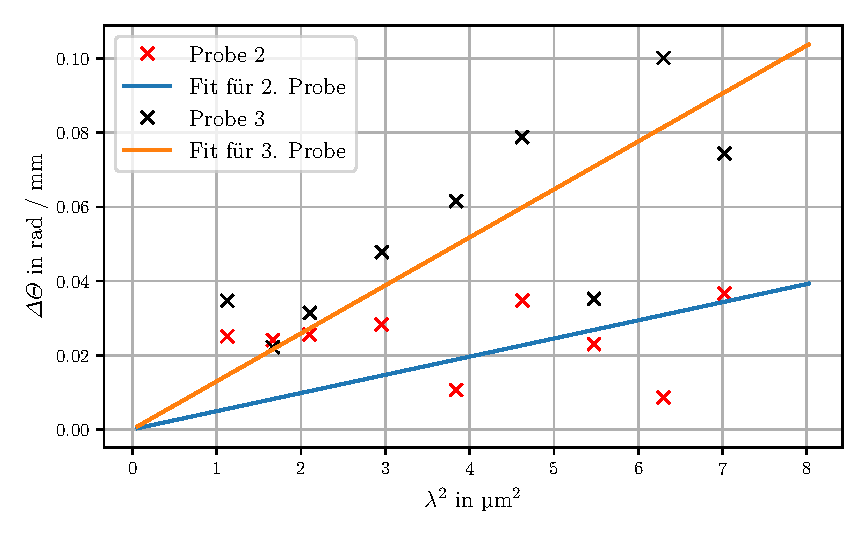
\includegraphics{build/probe23.pdf}
  \caption{Abgebildet sind die berechneten $\Delta\theta$ über dem Quadrat der Wellenlängen $\lambda^2$ der Filter. Für beide Proben ist eine lineare Ausgleichsrechnung eingezeichnet.}
  \label{fig:plot23}
\end{figure}

Desweiteren wird der Brechungsindex $n$ der verschiedenen Filter betrachtet. Die Brechungsindizes sind in Tabelle \ref{tab:n} aufgelistet. Für die folgende Bestimmung der effektiven Masse wird der Mittelwert
der Brechungsindizes verwendet:
\begin{align}
  n = \SI{3.36(5)}{}
\end{align}

Mit dem Parameter $A$ aus der Ausgleichsrechnung lässt sich die effektive Masse bestimmen:
\begin{align}
  (m^*)^2 = \frac{NB\mathrm{e}_0^3}{8\pi^2\epsilon_0\mathrm{c}_0^3nA}
\end{align}
Dabei steht $\mathrm{e}_0$ für die Elementarladung, $\mathrm{c}_0$ für die Lichtgeschwindigkeit im Vakuum und
$\epsilon_0$ für die Elektrische Feldkonstante.

Es ergibt sich für die zwei dotierten Proben:
\begin{align}
  m^*_2 &= \SI{8(1)e-32}{\kilogram}\\
  m^*_3 &= \SI{7.7(4)e-32}{\kilogram}
\end{align}

Das Verhältnis aus effektiver Masse und Ruhemasse $m_0$ ergibt sich zu
\begin{align}
  \frac{m^*_2}{m_0} &= \SI{0.089(10)}{}\\
  \frac{m^*_3}{m_0} &= \SI{0.084(5)}{} 
\end{align}

\begin{table}
  \centering
  \begin{tabular}{c c}
    \toprule
    $\lambda$ / $\SI{}{\micro\metre}$ & $n$\\
    \midrule
        1,06  & 3,4744\\  
        1,29  & 3,4078\\  
        1,45  & 3,3820\\  
        1,72  & 3,3551\\  
        1,96  & 3,3404\\  
        2,16  & 3,3323\\  
        2,34  & 3,3261\\  
        2,51  & 3,3217\\  
        2,65  & 3,3187\\  
    \bottomrule
  \end{tabular}
  \caption{Die Wellenlängen $\lambda$ der Filter und die
  Brechungsindizes $n$ \cite{rii}.}
  \label{tab:n}
\end{table}

